%% -*- coding:utf-8 -*-

\settowidth\jamwidth{(German)}


\chapter{Phenomena}


This chapter deals with variation in the Germanic languages in what is often called the Core
Grammar, that is in sentences of the \emph{John loves Mary} variety.\footnote{%
  \citet[\page 7--8]{Chomsky81a} suggests dividing grammars of natural languages into a core part and a periphery.
All regular parts belong to the core. The core grammar of a language is assumed to be an instance of
Universal Grammar (UG), the genetically determined innate language faculty of human beings. Idioms
and other irregular parts of a language belong to the periphery. This book deals with phenomena
usually assumed to be the core without assuming this core/periphery distinction and without assuming
an UG \citep{MuellerKernigkeit,MuellerCoreGram}.
} We will look at differences in
the verb position (verb before object and object before verb), the verb second property, which
all of the Germanic languages with the exception of English have, the ordering of subjects and
obejcts with respect to each other, the placement of adverbials, the existence/non-existence of
verbal complexes, the obligatoriness/absence of subjects, passive including the personal and
impersonal passive, expletive pronouns and various ways to mark the clause type.

A note of caution is necessary here: especially the following three subsections are potentially
confusing. A language like German will be categorized as an Subject-Object-Verb language, a verb-second language and
a language with free constituent order \citep{Haftka96a}. This sounds contradictory but it is not. The respective
classifications refer to properties of languages as such not to the form of single sentences.

\section{Order of subject, object and verb}
\label{sec-intro-svo}

The langauges of the world can be classified according to the order of subject, object, and verb
that is dominant \citep{Greenberg63a-u}. In order to make languages comparable a very general definition of grammatical
functions like subject and object is used
for such a classification. The definition is based on semantic properties: subjects are those
arguments that are agentlike and objects are arguments that are rather patient like. This definition
is not always identical to the language-particular definitions. For instance, if one follows the
semantic definition, the phrase \emph{der
  Aufsatz} `the paper' in (\mex{1}) is the subject although it is inanimate and not an agent: 
\ea
\gll Der Aufsatz interessiert mich.\\
     the paper   interests    me\\
\glt `I am interested in the paper.'
\z
The language-particular definition of subject in German (and the Germanic languages in general)
rather refers to properties like nominative case, subject-verb-agreement, and control. We will deal with this in more
detail in Section~\ref{sec-subj-properties}.

Figure~\vref{fig-sov-wals} shows the dominant order of subject, object, and verb among the world's languages.
\begin{figure}[htbp]
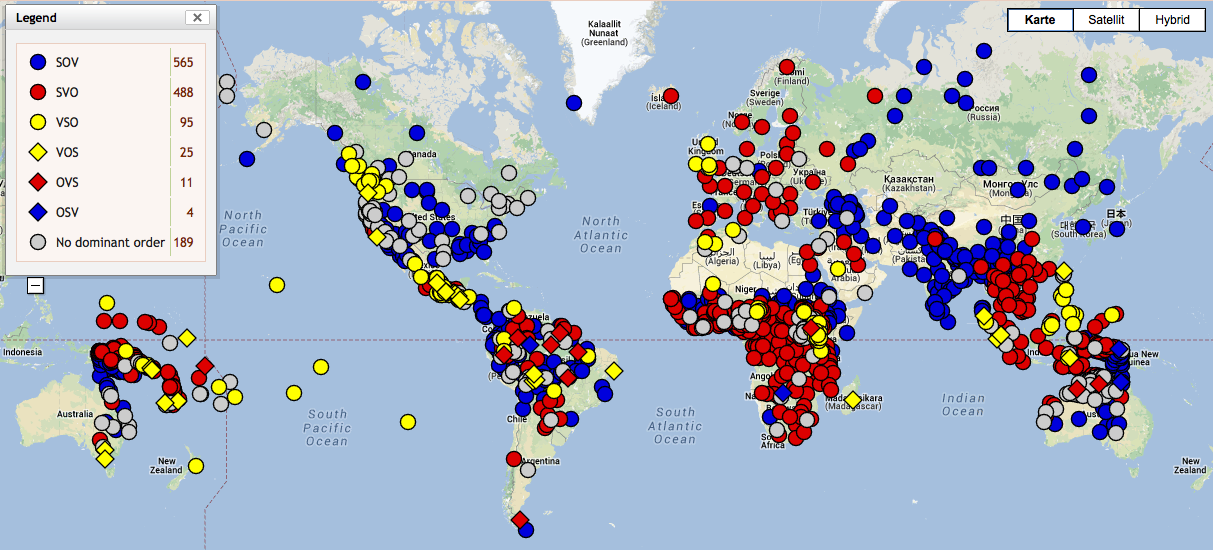
\includegraphics[width=\textwidth]{Pictures/WALS-SOV}
\caption{\label{fig-sov-wals}Matthew S.\ Dryer: Feature 81A: Order of subject, object and verb, The World Atlas of Language Structures} 
\end{figure}
According to \citet{Dryer2013a} the dominant order is defined as follows:

%Dominante Abfolge (Dryer: Determining Dominant Word Order):
\begin{quote}
Where a language is shown on one of the word order maps as having a particular order as the dominant
order in the language, this means that it is either the only order possible or the order
that is more frequently used. \citep{Dryer2013a}
\end{quote}
%
%% I base my classification of Macushi here on the frequency counts, and since no order is more than
%% twice as frequent as the next most frequent order, I treat this language as lacking a dominant order
%% of subject, object, and verb.
%
%% Deutsch, Niederländisch und Friesisch sind V2-Sprachen, that is die SVO- und SVAuxOV-Stellungen kommen
%% durch die Voranstellung des Verbs zustande, die eine Funktion hat. Wir zählen diese Sprachen also
%% mit zu den SOV-Sprachen.
%
If we zoom in to display the European languages we get Figure~\vref{fig-sov-wals-europe}.
\begin{figure}[htbp]
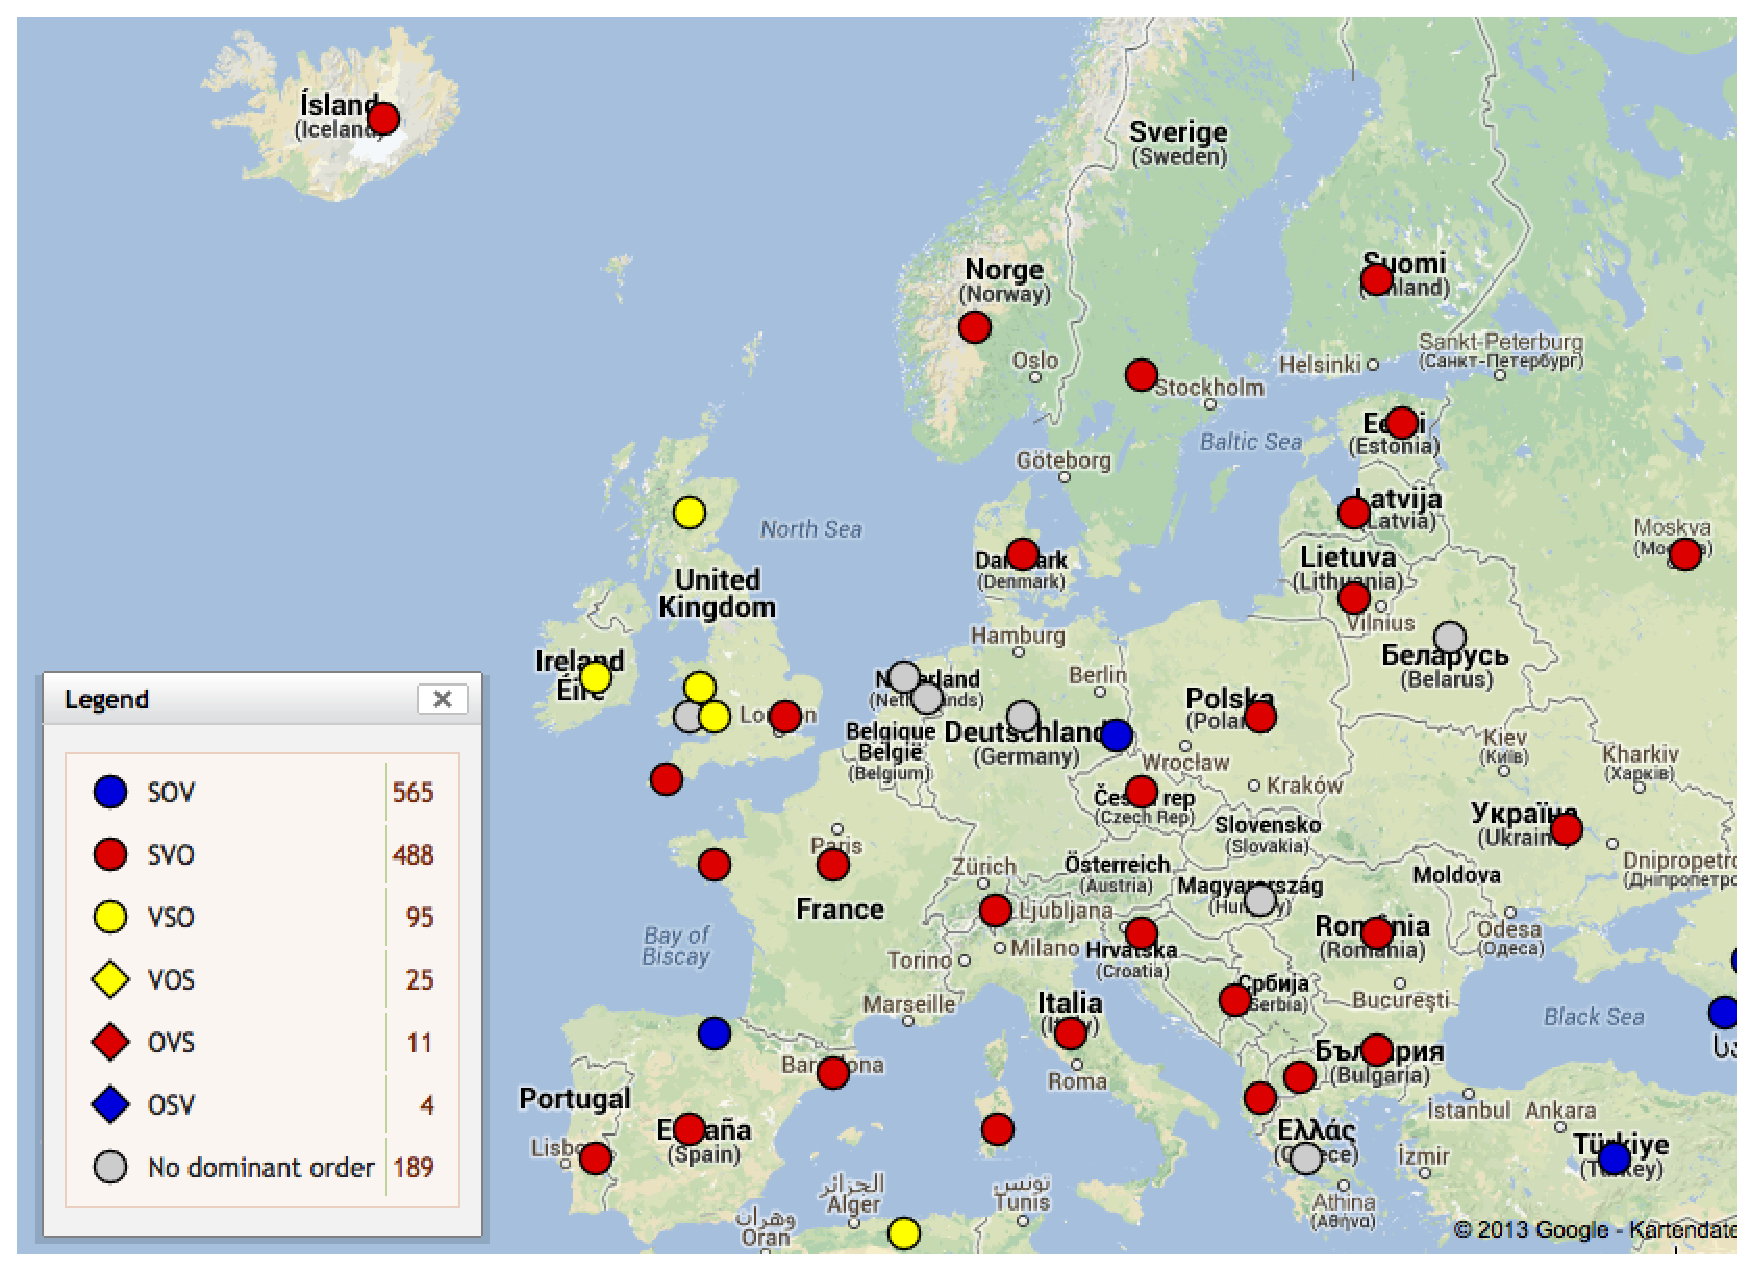
\includegraphics[width=.898\textwidth]{Pictures/WALS-SOV-Europa}
\caption{\label{fig-sov-wals-europe}Dominant orders of subject, object, and verb in Europe}
\end{figure}
According to the WALS the languages Iclandic, Norwegian, Swedish, Danish, and English are SVO
languages. Dutch, German, and Frisian, however, are marked in grey, that is, these languages are
marked to have no dominant order.\footnote{
  \citet[\page 87]{Greenberg63a-u} listed German and Dutch among the SVO languages.%
} According to Figure~\vref{fig-sov-wals-europe-two} these languages
have two dominant orders, namely SOV and SVO.
\begin{figure}[htbp]
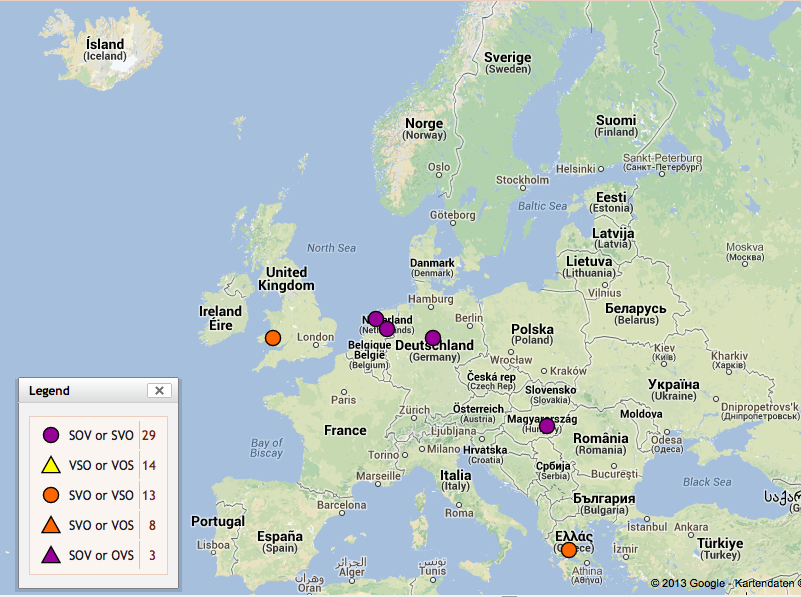
\includegraphics[width=.898\textwidth]{Pictures/WALS-SOV-Europa-no-dominant}
\caption{\label{fig-sov-wals-europe-two}%Dryer: Feature 81b: 
Two dominant orders of subject, object, and verb}
\end{figure}
The reason for this classification is that Dryer distinguishes between sentences in which the finite
verb is the main verb (\mex{1}a) and sentences in which the finite verb is an auxiliary as in (\mex{1}b):
\eal
\ex 
\gll Kim sieht den Mann.\\
     Kim gees the man\\
\glt `Kim sees the man.'
\ex
\gll Kim hat den Mann gesehen.\\
     Kim has the man seen\\
\glt `Kim has seen the man.'
\zl
According to Dryer the pattern for (\mex{0}a) is SVO and the one for (\mex{0}b) is SAuxOV, where Aux
stands for the auxiliary verb. Like
\citet{Greenberg63a-u}, Dryer counts the latter pattern as SOV order. The question is whether it is adequate to ignore auxiliaries
in the examination of constituent order. The auxiliary \emph{hat} `have' in (\mex{0}b) syntactically
behaves like the full verb \emph{scheint} `seems' in (\mex{1}):
\ea
\gll Kim scheint den Mann zu sehen.\\
     Kim seems   the man  to see\\
\glt `Kim seems to see the man.'
\z
So, here we would have an SVOV order, something that does not exist in the typology under discussion.
The languages in Figure~\ref{fig-sov-wals-europe-two} marked as not having a dominant order use the
verb position to mark the clause type: it is just the finite verb that is in first or second
position. Non-finite verbs are final: 
\ea
\gll Kim scheint den Mann gesehen zu haben.\\
     Kim seems   the man  seen to have\\
\glt `Kim seems to have seen the man.'
\z
In subordinate clauses we have both the finite verb and the non-finite verbs in final position while
we have the finite verb in initial position\footnote{%
  I use the term initial position to refer to the position the finite verb has in V1 or V2 clauses. The
  analysis of V2 and V1 involves fronting of the finite verb. In V2 clauses a constituent is fronted
  in addition.
} in questions and declarative main clauses.
A classification that is entirely based on counting patterns without taking auxiliary verbs into
account cannot tear these properties apart \citep{Hoehle83a}. In what follows we will have a look at clauses with
both finite and non-finite verbs. Such clauses reveal differences between OV and VO languages and I will argue that Afrikaans, Dutch,
German, and Frisian should be counted among the OV languages and that the other observable pattern
SVO is due to other properties of these languages, namely that they mark the clause type by verb
position and that they are verb second (V2) languages.\footnote{%
  The property of being a V2 language is independent of the SVO/SOV distinction. All Germanic
  languages except English are V2 languages. See Section~\ref{sec-phenomenon-v2} on V2.
}

When one builds more complex German sentences involving several verbs, the embedding verb is usually
realized to the right of the embedded verbs. This is shown in (\mex{1}). (\mex{1}a) shows a simple
sentence with a finite verb. If we form the perfect as in (\mex{1}b), the perfect auxiliary has to
follow the participle. The auxiliary is the finite verb and it determines the form of the
participle. Hence the finite verb is the verb that embeds the participle. This is indicated by the
lower number of \emph{hat} in comparison to \emph{gesehen}. If we build an even more complex
sentence by adding another verb, this verb will be serialized to the right of the present verbs
(\mex{1}c).  The Danish example in (\mex{2}c), quoted from \citet{Oersnes2009b}, corresponds to the
German example in (\mex{1}c).

\eal
\ex
\gll dass er ihn sieht$_1$\\
     that he him sees\\\jambox{(German)}
\glt `that he sees him'
\ex
\gll dass er ihn gesehen$_2$ hat$_1$\\
     that he him seen        has\\
\glt `that he has seen him'
\ex
\gll dass er ihn gesehen$_3$ haben$_2$ muss$_1$\\
     that he him seen        have     must\\
\glt `that he must have seen him'
\zl
\eal
\ex
\gll at   han ser$_1$ ham\\
     that he  sees    him\\\jambox{(Danish)}
\ex
\gll at   han have$_1$ set$_2$ ham\\
     that he  has      seen    him\\
\ex
\gll at   han må$_1$ have$_2$ set$_3$ ham\\
     that he  must   have     seen   him\\
\zl
%
As the examples in (\mex{0}) show, the verbs are added in front of the verbs they embed in
Danish. This is also the case for English as is evident from the glosses. In Danish and English the
verbs precede the object (\emph{ham}/\emph{him}) and in German they follow it (\emph{ihn}). 

\citet{Haider2017b-u} pointed out two further differences between the Germanic VO and OV languages:
particles precede verbs in OV languages and the same is true for resultative secondary
predicates. In VO languages particles and result predicates follow the verb. This is demonstrated by
the following two example sets:
\eal
\ex Peter will look up the information.
\ex 
\gll Peter wird die Information nachschlagen.\\
     Peter will the information \textsc{part}.beat\\\jambox{(German)}
\glt `Peter will look up the information.'
\zl
\eal
\ex Peter will fish the pond empty.
\ex 
\gll Peter wird den Teich leer fischen.\\
     Peter will the pond  empty fish\\\jambox{(German)}
\zl
(\mex{-1}a) shows that \emph{look} precedes the particle \emph{up}, while the verb \emph{schlagen}
`beat' has to follow the particle \emph{nach} in German. Similarly, the secondary resultative
predicate \emph{empty} follows the verb in (\mex{0}a), but \emph{leer} precedes the verb in
(\mex{0}b). Note that I used a future auxiliary in the examples in order to avoid side effects that
are due to the verb second property of German: in declarative main clauses the finite verb always
precedes particles and resultative predicates but this is due to the clause type (see Section~\ref{sec-phenomenon-v2}).

I will return to the SVO vs.\ SOV order in Chapter~\ref{chap-verb-position} and provide more
evidence that was used in the literature to argue for the OV status of languages like German and Dutch.


\section{V2}
\label{sec-phenomenon-v2}

The Germanic languages, with the exception of English, are so-called \emph{verb second languages} (V2
languages). The V2
property can be illustrated with the following German sentences. (\mex{1}) shows declarative main
clauses in which one of the constituents is fronted. (\mex{2}) shows parallel interrogative clauses.

\eal
\ex 
\gll Der Mann gibt der Frau morgen das Buch.\\
     the man  gives the woman tomorrow the book\\\jambox{(German)}
\glt `The man give the woman the book tomorrow.'
\ex 
\gll Der Frau gibt der Mann morgen das Buch.\\
     the woman gives the man tomorrow the book\\
\ex 
\gll Das Buch gibt der Mann der Frau morgen.\\
     the book gives the man the woman tomorrow\\
\ex 
\gll Morgen gibt der Mann der Frau das Buch.\\
     tomorrow gives the man the woman the book\\
\zl
\eal
\ex 
\gll Wer gibt der Frau morgen das Buch?\\  
     who gives the woman tomorrow the book\\\jambox{(German)}
\glt `Who gives the woman the book tomorrow?'
\ex 
\gll Wem gibt der Mann morgen das Buch?\\
     who gives the man tomorrow the book\\
\glt `Who does the man give the book to?'
\ex 
\gll Was gibt der Mann der Frau morgen?\\
     what gives the man the woman tomorrow\\
\glt `What does the man give the woman?'
\ex 
\gll Wann gibt der Mann der Frau das Buch?\\
     when gives the man the woman the book\\
\glt `When does the man give the woman the book?'
\zl
The finite verb is in second position in all the sentences in (\mex{-1}) and (\mex{0}).


English, in contrast, does not allow orders in which the object appears immediately before the
finite verb.

\eal
\ex[*]{ 
This man give I a book tomorrow.
}
\ex[*]{
This book give I a man tomorrow.
}
\ex[*]{
Tomorrow give I the man a book.
}
\zl 
Adverbials and objects can be fronted but then they have to appear before the clause consisting of
subject and verb and possibly other constituents.
\eal
\ex This book, I give the man tomorrow. 
\ex Tomorrow, I give the man a book.
\zl

Note also that fronting of objects is restricted to the secondary object for verbs with two objects
for some speakers \citep[\page 258]{Hudson92a-u}.\footnote{
  I use the terms \emph{primary object}\is{object!primary} and \emph{secondary object}\is{object!secondary} in order to avoid confusion that is sometimes
  caused by the terms \emph{direct}\is{object!direct} and \emph{indirect object}\is{object!indirect}. The primary object is the first object in English
  and the dative object of ditransitive verbs governing the dative in German. The secondary object
  is the second object in English and the accusative in German ditransitive constructions.
} So, while fronting of the secondary object in
(\mex{1}b) is permitted by all speakers, some speakers find extractions like the extraction of the
primary object in (\mex{1}c) unacceptable or marked.
\eal
\judgewidth{\%}
\ex[]{
We give children sweets.
}
\ex[]{
These sweets, we give children \_.
}
\ex[\%]{
These children, we give \_ sweets.
}
\zl
This is not the case in V2 languages: they are rather liberal as far as fronting
is concerned. Basically all constituents can be fronted, exceptions being reflexive
pronouns that are selected by inherently reflexive verbs (\mex{1}), expletive objects (\mex{2}), and certain modal
particles (\mex{3}).\todostefan{references}
\eal
\ex[]{
\gll Maria erholt sich.\\
     Maria recovers \refl\\\german
\glt `Maria recovers.'
}
\ex[*]{
\gll Sich erholt Maria.\\
     \refl{} recovers Maria\\
}
\zl
\eal
\ex[]{
\gll Er bringt es bis zum Professor.\\
     he brings \expl{} until to.the professor\\\german
\glt `He makes it to professor.'
}
\ex[\#]{
\gll Es bringt er bis zum Professor.\\
     \expl{} brings he until to.the professor\\
} 
\zl
\eal
\ex[]{
\gll Er geht halt nicht.\\
     he goes \textsc{particle} not\\\german
\glt `He simply does not go.'
}
\ex[*]{
\gll Halt geht er nicht.\\
     \textsc{particle} goes he not\\
}
\zl

The element in front of the finite verb is not necessarily a clause mate of the finite verb. In
fact, it can belong to a deeply embedded head as is demonstrated by the following example from
German:
\ea
\gll [Über dieses Thema]$_i$ habe ich ihn gebeten, [[einen Vortrag \_$_i$ zu halten]?\footnotemark\\
     \spacebr{}about this topic  have I him asked \hspaceThis{[[}a talk {} to hold\\\german
\footnotetext{
\citew[\page 21]{HN89b}.
}
\glt `I asked him to give a talk about this topic.'
\z
The PP \emph{über dieses Thema} depends on \emph{Vortrag} `talk', which is part of the VP headed by
\emph{zu halten} `to hold', which is in turn embedded under \emph{gebeten} `asked'. Sentences like
(\mex{0}) show that V2 frontings cannot be analyzed as a simple reordering of the arguments of a
verb. While such an approach would work for the examples in (\mex{1}), it would not extend to other
cases in which the fronted element does not depend on the highest verb in the clause.
\ea
\gll Den Mann kennt er.\\
     the.\acc{} man knows he\\
\glt `He knows the man.'
\z

The following examples from Danish (SVO) show that the property of being a V2
language is independent of the VO/OV property:
\eal
\ex 
\gll Max har læst bogen.\\
     Max has read book.\textsc{def}\\\danish
\ex
\gll Bogen har Max læst.\\
     book.\textsc{def} has Max read\\
\zl
The example in (\mex{0}a) shows that the object follows the verbs and (\mex{0}b) shows that the
object \emph{bogen} `the book' can appear in sentence initial position infront of the finite verb
\emph{har} `have'.

The V2 order is used in declarative main clauses throughout the Germanic languages (without
English). Some Germanic languages do not use V2 order in embedded clauses. For a discussion of
embedded interrogatives see Section~\ref{sec-embeeded-clauses}.

While English does not allow for the order object verb subject, which is possible in the other Germanic
languages due to V2 fronting, it allows for the fronting of the object in questions resulting in
structures that are parallel to what we know from the other Germanic languages:
\eal
\ex Which book did Peter read?
\ex Which book did Peter give to Mary?
\ex To whom did Peter give the book?
\zl
English used to be a V2 language but lost this property. The V2 in questions is a residue of earlier
stages of the language, which is why English is called a \emph{residual V2 language}\is{V2
  language!residual} \citep{Rizzi1990a-u}. 

V2 and verb fronting in general is a way to mark clause types in all Germanic languages. V2 sentence
can be declarative clauses in all Germanic languages except English and they can be questions in all
Germanic languages including English. In addition V2 sentences may be imperatives, as (\mex{1}) shows.
\ea
\gll Jetzt gib ihm das Buch!\\
     now give me the book\\\german
\glt `Give me the book now!'
\z
Sentences with the finite verb in first position (V1) can be yes/no questions or imperatives:
\eal
\ex
\gll Gibt er ihm das Buch?\\
     gives he him the book\\\german
\glt `Does he give him the book?'
\ex 
\gll Gib mir das Buch!\\
     give me the book\\
\zl
Of course the order of elements is not the only cue as far as the clause type is
concerned. Intonation and morphological marking of imperative forms plays a role as well.

The property of being a V2 language is sort of perverse: it is exceedingly rare among the world's
languages.\todostefan{add references} Apart from the Germanic languages there are only Modern Breton, Old French, Kashmiri, the
austronesian languages Taiof and Sisiqa, the brazilian native languages Karitiana from the language
family Tupí and the uto-aztekian language Tohono O'odham, which is spoken in the southwest of the US
and in northern Mexico.


\section{Scrambling}

While the constituent order in languages like English is rather fixed, languages like Dutch and
German allow a rather free permutation of arguments. In order not to contaminate the effects by
reorderings that are due to the V2 property, I use verb last sentences to illustrate the
phenomenon. Example (\mex{1}) shows the only possible order for subject and objects of a simple
ditransitive sentence without extraction:


\ea
because the man gives the woman the book \jambox{(English)}
\z
If speakers want to realize the secondary object \emph{the book} before the primary object \emph{the
  woman}, they have to use a prepositional object. This type of reordering is called
\emph{dative-shift} and an example is provided in (\mex{1}):
\ea
because the man gives the book to the woman \jambox{(English)}
\z
In contrast to this we have the German examples in (\mex{1}). These examples show that the noun
phrases can be freely permuted:
\eal
\ex 
\gll {}[weil]          der Mann der Frau das Buch gibt\\
     \spacebr{}because the man the woman the book gives\\\jambox{(German)}
\ex 
\gll {}[weil]          der Mann das Buch der Frau  gibt\\
     \spacebr{}because the man  the book the woman gives\\
\ex 
\gll {}[weil]          das Buch der Mann der Frau  gibt\\
     \spacebr{}because the book the man  the woman gives\\
\ex 
\gll {}[weil]          das Buch der Frau  der Mann gibt\\
     \spacebr{}because the book the woman the man  gives\\
\ex 
\gll {}[weil]          der Frau  der Mann das Buch gibt\\
     \spacebr{}because the woman the man  the book gives\\
\ex 
\gll {}[weil]          der Frau  das Buch der Mann gibt\\
     \spacebr{}because the woman the book the man  gives\\
\zl
Not all of these orders can be used in all contexts. Some of the examples require a special,
contrastive intonation. The orders can be sorted with respect to the number of contexts in which
they can be used. \citet{Hoehle82} suggests calling the order that can be used in most contexts the
normal or unmarked order.




\section{The position of adverbials}


In languages like German, the position of adverbials is rather free: the adverb \emph{gestern}
`yesterday' can appear anywhere between the arguments and the verb:\todostefan{add Dutch examples}
\eal
\ex
\gll weil der Mann der Frau das Buch {gestern} gab\\ 
     because the man the woman the book yesterday gave\\\jambox{(German)}
\glt `because the man gave the woman the book yesterday'
\ex 
\gll weil der Mann der Frau {gestern} das Buch gab\\
     because the man the woman yesterday the book gave\\
\ex 
\gll weil der Mann {gestern} der Frau das Buch gab\\
     because the man yesterday the woman the book gave\\
\ex 
\gll weil {gestern} der Mann der Frau das Buch gab\\
     because yesterday the man the woman the book gave\\
\zl

In contrast, the position of the adverbials is rather restricted in SVO languages like Danish and
English. The adverbials usually are placed before or after the VP; that is, verb and objects form one
unit and adverbials attach to the left or to the right of this unit. (\mex{1}) provides an example:
\eal
\ex[]{
because the man {often} [gave the woman the book] \jambox{(English)}
}
\ex[]{
because the man [gave the woman the book] {often}
}
\ex[*]{
because the man [gave often the woman the book]
}
\ex[*]{
because the man [gave the woman often the book]
}
\zl
It is assumed that verb and objects form a structural unit, a verb phrase (VP). Adverbials may
attach to this VP forming a larger VP, which is than combined with the subject to form a complete sentence.

The following example, which is due to \citet[§ 8.20, 495]{QGLS85a-u}, shows that even in very
complex combinations of several verbs adverbs may be placed at the left periphery of a VP:
\ea
It [certainly [\sub{VP} may [possibly [\sub{VP} have [indeed [\sub{VP} been\\ {}[badly [\sub{VP} formulated]]]]]]]].
\z
This is different from the OV languages where verbs form a verbal complex which usually cannot be
interrupted by adverbs.
\eal
\ex[]{
\gll dass der Mann der Frau das Buch morgen geben dürfen muss\\
     that the man  the woman the book tomorrow give may must\\
\glt `that it must be possible that it is allowed that the man gives the woman the book tomorrow'
}
\ex[*]{
\gll dass der Mann der Frau das Buch geben morgen dürfen muss\\
     that the man  the woman the book give tomorrow may must\\
}
\ex[*]{
\gll dass der Mann der Frau das Buch geben dürfen morgen muss\\
     that the man  the woman the book give  may tomorrow must\\
}
\zl

\section{Embedded clauses}
\label{sec-embeeded-clauses}

This section deals with embedded clauses that are introduced by a complementizer and with
embedded interrogative clauses. The Germanic languages vary with respect to the verb placement in
these subordinate clauses and with respect to the question whether the embedded clauses are V2 or not.

\subsection{Embedded clauses introduced by a complementizer}

As was already mentioned Afrikaans, Dutch, German are SOV languages and this is shown in embedded
clauses that are introduced by a complementizer. (\mex{1}) is an example:

\ea
\gll Ich weiß, dass Max das Buch heute gelesen hat.\\
     I know that Max the book today read has\\
\glt `I know that Max read the book today.'
\z


%% Stellung der anderen Konstituenten ist frei:
%% \eal
%% \ex Ich weiß, dass das Buch Max heute gelesen hat.
%% \ex Ich weiß, dass das Buch heute Max gelesen hat.
%% \zl

English, beeing an SVO non-V2 language allows for SVO order only.
\ea[]{
I  know that Max has read the book yesterday. \jambox{(English)}
}
\z

Interestingly, Danish, also an SVO languauge, allows both SVO order (\mex{1}) and V2 order (\mex{2}) in clauses
preceeded by a complementizer:
\ea[]{
\label{ex-at-max-ikke-har}
\gll Jeg  ved, at   Max ikke  har læst   bogen          {i dag}.\\
     I know that Max not has read book.\textsc{def} today\\\jambox{(Danish)}
\glt `I know that Max did not read the book today.'
}
\z
%(Negation hilft, Verbstellung zu bestimmen)

\eal
\ex[]{
\gll Jeg  ved, at   {i dag} har Max ikke læst bogen.\\
     I    know that today   has Max not read book.\textsc{def}\\\jambox{(Danish)}
}
\ex[]{
\gll Jeg  ved, at   bogen          har Max ikke  læst {i dag}.\\
     I know that book.\textsc{def} has Max not read today\\
}
\zl
The example in (\ref{ex-at-max-ikke-har}) includes the negation in order to show that we indeed deal
with the SVO order here. Without the negation it is not clear whether non-V2 clauses are allowed in
clauses that are introduced by a complementizer since (\mex{1}a) has the finite verb in second
position. With the negation present, it is clear that we have a V2 clause if the negation follows
the finite verb and that we do not have a V2 clause if the finite verb follows the negation as in
(\mex{-1}) and hence is in third position.
\eal
\settowidth\jamwidth{(V2 or SVO)}
\ex 
\gll at Max har læst bogen\\
     that Max has read book.\textsc{def}\\\jambox{(V2 or SVO)}
\ex 
\gll at Max har ikke læst bogen\\
     that Max has not read book.\textsc{def}\\\jambox{(V2)}
\zl 
For complementizerless sentences the V2 order is the only one that is possible:
\eal
\settowidth\jamwidth{(V2 or SVO)}
\ex[]{ 
\gll Max har ikke læst bogen\\
     Max has not read book.\textsc{def}\\\jambox{(V2)}
}
\ex[*]{ 
\gll Max ikke har læst bogen\\
     Max not  has read book.\textsc{def}\\\jambox{(SVO)}
}
\zl 


Yiddish and Icelandic are SVO languages as well. The clauses that are combined with a
complementizer are V2:
\eal
\ex
\gll Ikh meyn  az   haynt hot Max geleyent dos bukh.\footnotemark\\
     I think that today has Max read the book\\\yiddish
\footnotetext{\citew[p.\,58]{Diesing90a}.}
\glt `I think that Max read the book today.'

\ex% check!
\gll Ikh meyn  az   dos bukh hot Max geleyent.\\
     I think that the book has Max read\\

\zl
\todostefan{provide Icelandic example}


\subsection{Interrogative clauses}


The OV languages form subordinated interrogative clauses by preposing a phrase containing an
interrogative pronoun\footnote{
Most interrogative pronouns start with \emph{w} in German and \emph{wh} in English. Phrases
containing an interrogative pronoun are called \emph{w} phrases or \emph{wh} phrases,
respectively. Interrogative clauses are sometimes called \emph{w} clauses or \emph{wh} clauses.
} from an
otherwise SOV clause. (\mex{1}) shows a German example:
\eal
\ex 
\gll Ich weiß, wer heute das Buch gelesen hat.\\
     I know    who today the book read has\\\jambox{(German)}
\glt `I know who read the book today.'
\ex 
\gll Ich weiß, was Max heute gelesen hat.\\
     I know    what Max today read has\\
\glt `I know what Max has read today.'
\zl
Since languages like German allow for scrambling, senteces like those in (\mex{0}) could just be due
to the permutation of arguments of a head. However, the generalization about these \emph{w} clauses
is that an arbitrary \emph{w} element can be fronted. (\mex{1}) gives an example from German that
involves a nonlocal dependency:
\ea
\gll Ich weiß nicht, [über welches Thema]$_i$ er versprochen hat,~~~~~~~~ [[einen Vortrag \_$_i$] zu halten].\\
     I know not      \spacebr about which topic he promised has \hspaceThis{[[}a talk to  hold\\\jambox{(German)}
\glt `I do not know about which topic he promised to give a talk.'
\z
Here, the phrase \emph{über welches Thema} `about which topic' is an argument of \emph{Vortrag},
which is embedded in the VP containing \emph{zu halten} `to hold', which is in turn embedded under
\emph{versprochen hat} `promised has'. The generalization about interrogative clauses is that an
interrogative clause consists of a interrogative phrase (\emph{über welches Thema} `about which
topic') and a clause in which this interrogative phrase is missing somewhere (\emph{er versprochen
  hat, einen Vortrag zu halten} `he promised to give a talk').

In German the order of the other constituents is free as in assertive main clauses and embedded
clauses with a complementizer that were discussed earlier. 
\eal
\ex
\gll Ich weiß, was keiner diesem Mann geben würde.\\
     I know    what nobody this man give would\\\jambox{(German)}
\glt `I know what nobody would give this man.'
\ex 
\gll Ich weiß, was diesem Mann keiner geben würde.\\
     I know what this man nobody give would\\
\zl

In Danish and English the interrogative clauses consist of an interrogative phrase and an SVO clause
in which it is missing:
\eal
\ex 
\gll Max har givet ham bogen.\\
     Max has given him book.\textsc{def}\\\jambox{(Danish)}
\glt `Max gave him the book.'
\ex
\gll Jeg ved, hvad$_i$ [Max har givet ham \_$_i$].\\
     I know what \spacebr{}Max has given him\\
\glt `I know what Max gave him.'
\ex
\gll Jeg ved, hvem$_i$ [Max har givet \_$_i$   bogen].\\
     I know who        \spacebr{}Max has given {} book.\textsc{def}\\
\glt `I know who Max has given the book.'
\zl
(\mex{0}a) shows the clause with SVO order and (\mex{0}b) is an example with the secondary object as
interrogative ponoun and (\mex{0}c) is an example with the primary object as interrogative
pronoun. The position that the respective objects have in non-interrogative clauses like (\mex{0}a)
is marked with \_$_i$.

Yiddish is special in that it has a V2 order in interrogative clauses as well \citep[Sections~4.1, 4.2]{Diesing90a}: interrogatives
consist of a interrogative phrase that is extracted from a V2 clause:

\ea
\gll Ir veyst efsher [avu            do    voynt Roznblat   der goldshmid]?\footnotemark\\
     you know maybe  \spacebr{}where there lives Rosenblatt the goldsmith\\
\glt `Do you perhaps know where Rosenblatt the goldsmith lives?' 
\footnotetext{
\citew[S.\,65]{Diesing90a}. Zitiert aus Olsvanger, \emph{Royte Pomerantsn}, 1949
}
\z

%% \eal 
%% \ex
%% \label{vosmaks}
%% \gll Ikh veys nit   vos$_i$ [Max hot gegesn \_$_i$].\footnotemark\\
%%      I know not     what \hspaceThis{[}Max has eaten\\
%% \footnotetext{\citew[p.\,68]{Diesing90a}.}
%% \glt `I do not know what Max has eaten.'

%% \ex%check
%% \gll Ikh veys nit   [vos                    hot Max gegesn].\footnotemark\\
%%      ich weiß nicht \hspaceThis{[}was heute hat Max gegessen\\
%% \footnotetext{\citew[S.\,68]{Diesing90a}.}
%% \glt `Ich weiß nicht, was Max heute gegessen hat.'
%\zl
So the variation is \emph{w}-phrase + SOV, \emph{w}-phrase + SVO, and \emph{w}-phrase + V2.


\section{The use of expletives to mark the clause type}

The Germanic languages use constituent order to code the clause type: V2 main clauses can be
assertions or questions, depending on the content of the preverbal material and
intonation. Similarly embedded interrogative clauses consist of a \emph{w} phrase and an SVO, SOV,
or V2 clause. The fronting of a constituent in a V2 clause comes with certain information structural
effects: something is the topic or the focus of an utterance. For embedded sentences it is important
for some languages that the structure is transparent that is that we have the \emph{w} + SVO or
\emph{w} + V2 order. There are situations in which it is inappropriate to front an element and in
such situations the Germanic languages use expletives, that is, pronouns that do not contribute
semantically, to maintain a certain order.

German uses the expletive \emph{es} to fill the position in front of the finite verb, if no other
constituent is to be fronted.
\eal
\ex 
\gll Drei Reiter ritten zum Tor hinaus.\\
     three riders rode  towards.the gate out\\\german
\glt `Three riders rode out of the gate.'
\ex 
\gll Es ritten drei Reiter zum Tor hinaus.\\
     \expl{} rode   three riders towards.the gate out\\
\zl

Danish uses the expletive to make it clear that an extraction of a consituent took place:
\eal
\ex[]{
\gll Politiet ved ikke, {hvem} der   havde placeret bomben.\\
     police.\textsc{def} knows not who \textsc{expl} has placed bomb.\textsc{def}\\
\glt `The police does not know who placed the bomb.'
}
\ex[*]{
\gll Politiet ved ikke, {hvem} havde placeret bomben.\\
     police.\textsc{def} knows not who has placed bomb.\textsc{def}\\
}
\zl
Without the expletive one would have a pattern like the one in (\mex{0}b). In (\mex{0}b) we have the
normal SVO order and it is not obvious to the hearer that the pattern consists of an extracted
element (the subject) and an SVO clause from which it is missing. This is more transparent if an
expletive is inserted into the subject position as in (\mex{0}a).

Similarly Yiddish uses an expletive in embedded interrogatives (\emph{w} + V2) if the subject is
extracted or if there is no other element that is information structurally appropriate for the preverbal position:
%% \ea
%% \label{vosmaks}
%% \gll Ikh veys nit   [vos Max hot gegesn].\footnotemark\\
%%      ich weiß nicht \hspaceThis{[}was Max hat gegessen\\
%% \footnotetext{\citew[S.\,68]{Diesing90a}.}
%% \glt `Ich weiß nicht, was Max gegessen hat.'
%% \z
%% 
%% \item 
(\mex{1}) shows examples from \citet{Diesing90a}:

\eal
\ex[]{
\gll ikh hob  zi  gefregt ver es         iz beser  far ir\\
     I   have her asked   who \textsc{expl} is better for her\\\yiddish
\glt `I have asked her who is better for her.'}
\ex[]{
\gll ikh hob  im  gefregt vemen es        kenen ale dayne khaverim\\
     I   have him asked   whom \textsc{expl} know  all your friends\\
\glt `I asked him whom all your friends know.'}
\zl
(\mex{0}a) is an example involving an interrogative pronoun that is the subject and (\mex{0}b) is an
example in which the preverbal position is not filled by an argument of \emph{kenen} `know' but by
an expletive. The subject \emph{ale dayne khaverim} `all your friends' stays behind and the object
\emph{vemen} `whom' is extracted since it is the interrogative pronoun.



\section{Verbal Complexes in OV languages}


The OV languages have a verbal complex, or more general, a predicate complex, since adjectives take
part in complex formation as well. (\mex{1}) gives a German example by \citew{Haider90b}:
\ea
\gll weil es ihm jemand zu lesen versprochen hat\\
     because it.\acc{} him.\dat{} somebody.\nom{} to read promised has\\\german
\glt `because somebody promised him to read it'
\z
The arguments of the respective verbs can be mixed with arguments of other verbs. In the example
above the \emph{es} `it' is not adjacent to its verb \emph{lesen} `to read', neither is \emph{ihm}
`him' adjacent to \emph{versprochen} `promised' nor \emph{jemand} to \emph{hat} `has'. In a more
``well-behaved'' ordering the object of \emph{zu lesen} `to read' is adjacent to the verb:
\ea
\gll weil    jemand   ihm das Buch zu lesen versprochen hat\\
     because somebody him the book to read  promised    has\\
\glt `because somebody promised him to read the book'
\z
The ordering in (\mex{0}) would allow for an analysis in which \emph{das Buch zu lesen} forms a VP
which is treated as an argument of \emph{versprochen} `promised'. However, this is not a viable
analysis for (\mex{-1}) if one assumes that phrases have to be continuous.

One explanation of orders like the one in (\mex{-1}) is that the verbs form a unit that behaves like a simplex verb. As with
the ditransitive verb \emph{geben} `to give' all permutations of the arguments of the verbs are
possible in principle. So \emph{zu lesen versprochen hat} forms a complex in both (\mex{-1}) and
(\mex{0}) and all permutations of the three arguments are permitted by the grammar.

VO languages like English and Danish do not allow permutations of arguments that belong to different
verbs. In VO languages governing verbs always embed VPs. The following example indicates the
structure:
\ea
because somebody [will [promise him [to read the book]]]
\z



\section{Obligatoriness of subjects, case of subjects, and passives}

SVO languages like English and Danish require a subject, while OV languages like German allow for
subjectless constructions.
\eal
\ex 
\gll Ihm graut vor der Prüfung.\\
     him.\dat{} dreads before the exam\\\german
\glt `He dreads the exam.'
\ex 
\gll Heute wird nicht gearbeitet.\\
     today is   not worked\\
\glt `There is no working today.'
\zl
According to the tests that were used for languages like Icelandic (for instance the possibility to
omit a subject in infinitival constructions), the dative object \emph{ihm} `him' in (\mex{0}a) is
not a subject. There is no nominal argument at all in (\mex{0}b). As we will discuss in
Section~\ref{sec-icelandic-quirky-subj}, Icelandic has dative subjects \citep{ZMT85a}, which makes it the most
exciting language to study among the Germanic languages. We will see that a uniform analysis of case
assignment is possible \citep*{YMJ87}, although there is some variety in the inflectional systems of the Germanic languages.


As is shown in (\mex{0}b), German allows for so-called impersonal passives. Impersonal passives are
a special kind of passives in which no element gets promoted to subject. SVO languages like English,
Danish do not allow subjectless constructions. English therefore does not allow impersonal passives
at all as (\mex{1}b) shows:
\eal
\ex[]{
\label{ex-gearbeitet-wurde}
\gll weil noch gearbeitet wird\\
     because still worked is\\\german
\glt `because there is still working there'
}
\ex[*]{
because (it) was worked \english
}
\zl
Interestingly, Danish found a way to fulfill the subject requirement and at the same time have
impersonal passives: Danish simply inserts an expletive pronoun into the subject position:
\eal
\label{ex-bliver-arbejder}
\ex 
\gll fordi der bliver arbejdet\\
     because \textsc{expl} is worked\\\danish
\glt `because there is working there'
\ex
\gll fordi   der arbejdes\\
     because  \textsc{expl} work.\textsc{pass}\\
\glt `because there is working there'
\zl
German does not allow for an expletive subject:
\ea[*]{
\gll  weil es noch gearbeitet wird\\
      because it still worked is\\\german
\glt `because there is still working there' 
}
\z
It is possible to have an expletive pronoun in front of the finite verb as in (\mex{1}), but this is
a positional expletive whose purpose it is to mark the V2 sentence type. 
\ea
\gll  Es wird noch gearbeitet.\\
      \textsc{expl} is still worked\\\german
\glt `There is still working there.'
\z
The expletive is not an argument of any verb. The purely positional character of this expletive is shown by the fact that it does not
appear in verb last sentences like (\mex{-1}).

\section{Summary}

This chapter provided an overview of the phenomena that are covered in this book. Of course we will
look at everything in much more detail in the chapters to come. Let's start and get our hands dirty.


\questions{

\begin{itemize}
\item What is the characteristics of a V2 language?
\item If a language has many sentences with subject, verb, object order, do you know that the language
  is a V2 language?
\end{itemize}

}




%      <!-- Local IspellDict: en_US-w_accents -->
